\section{Proof of Theorem~\ref{thm:main}}
\label{sec:characterisation}

We first identify exactly what subcubic homomorphism counts determine
on arbitrary graphs.
For a graph $G$ with adjacency matrix $A_G$, let
$W_G=\im A_G\subseteq\R^{V(G)}$.
For $d\in\{0,1,2,3\}$ and $f_1,\ldots,f_d\in\R^{V(G)}$, we define
\begin{equation}\label{eq:image-trilinear}
 \langle f_1,\ldots,f_d\rangle_G
 =\sum_{x\in V(G)}\prod_{i=1}^{d}f_i(x).
\end{equation}
The empty product is $1$, so $\langle\rangle_G=|V(G)|$.
The cases with one, two and three arguments are the linear form,
the standard inner product and the symmetric trilinear form, respectively.
We equip $W_G$ with the restricted inner product.

We use finite multigraphs, allowing loops and parallel edges; a loop
contributes two to the degree. For a multigraph $H$ and a tuple
$\mathbf m=(m_e)_{e\in E(H)}$ of positive integers, $H^{\mathbf m}$
is the subdivision that replaces each edge $e$ by a path of length $m_e$.
For a subdividing path with $q_e$ internal vertices, its length is $m_e=q_e+1$.
When every $m_e\geq3$, this subdivision is simple, even if $H$ has loops
or parallel edges.

Subdivision counts have an expansion in the spectral projectors of the target graph.
For a graph $G$ with adjacency matrix $A_G$, let $\Lambda_G$ be the set of
nonzero eigenvalues of $A_G$.
For $\lambda\in\Lambda_G$, $E_\lambda$ denotes the
$\lambda$-eigenspace and $P_\lambda$ its orthogonal projector.
For $\lambda\notin\Lambda_G$, including $\lambda=0$, we set
$E_\lambda=\{0\}$ and $P_\lambda=0$.
We add a graph subscript, as in $E_{\lambda,G}$ and $P_{\lambda,G}$,
when needed. For a multigraph $H$ and an edge labelling
$\ell:E(H)\to\R^\times$, the \emph{labelled coefficient} is
defined by
\begin{equation}\label{eq:contraction}
 c_G(H,\ell)=\sum_{\varphi:V(H)\to V(G)}
    \prod_{e=vw\in E(H)}P_{\ell(e)}(\varphi(v),\varphi(w)).
\end{equation}
For positive lengths making $H^{\mathbf m}$ simple,
\begin{equation}\label{eq:expansion}
 \hom(H^{\mathbf m},G)=\sum_{\ell:E(H)\to\Lambda_G}
       c_G(H,\ell)\prod_{e\in E(H)}\ell(e)^{m_e}.
\end{equation}
Indeed, for a path of length $m_e$ with endpoint images fixed at $x,y$,
summing over the images of its internal vertices gives
$A_G^{m_e}(x,y)=\sum_{\lambda\in\Lambda_G}\lambda^{m_e}P_\lambda(x,y)$.
Multiplying out these expansions over all edges gives \cref{eq:expansion}.
\begin{lemma}\label{lem:subdivision-coefficients}
For two graphs $G,G'$ and a multigraph $H$,
$\hom(H^{\mathbf m},G)=\hom(H^{\mathbf m},G')$ for every simple
subdivision $H^{\mathbf m}$ if and only if $c_G(H,\ell)=c_{G'}(H,\ell)$
for every edge labelling $\ell:E(H)\to\R^\times$.
\end{lemma}
\begin{proof}
Equality of the labelled coefficients gives equality of the counts by
\cref{eq:expansion}: since the coefficients vanish whenever a label
lies outside the target's nonzero spectrum, both sums may be taken over
$\ell:E(H)\to\Lambda_G\cup\Lambda_{G'}$.
Conversely, suppose the counts agree for every simple subdivision.
The functions $m\mapsto\lambda^m$ for
$\lambda\in\Lambda_G\cup\Lambda_{G'}$ are linearly independent on the
integers $m\geq3$, by the Vandermonde determinant.
Comparing the coefficients of $\prod_e\ell(e)^{m_e}$ in
\cref{eq:expansion} for $G$ and for $G'$, one variable $m_e\geq3$ at a time,
gives
$c_G(H,\ell)=c_{G'}(H,\ell)$ for every $\ell$.
\end{proof}

We call $G$ and $G'$ \emph{adjacency-image equivalent}, written
$G\sim_{\mathrm{im}}G'$, if $|V(G)|=|V(G')|$ and
there is a bijective linear map $U:W_G\to W_{G'}$ such that
\begin{equation}\label{eq:adjacency-image-equivalence}
 \begin{aligned}
 U(A_Gf)&=A_{G'}(Uf), &
 \langle Uf,Ug\rangle_{G'}&=\langle f,g\rangle_G, &
 \langle Uf,Ug,Uh\rangle_{G'}&=\langle f,g,h\rangle_G
 \end{aligned}
\end{equation}
for every $f,g,h\in W_G$.

A \emph{tensor} on a Euclidean space is a multilinear form, and its
\emph{coefficients} in a basis are its values on tuples of basis
vectors.
A \emph{closed tensor network} $\mathcal N$ is a finite multigraph with a tensor at
each vertex and one tensor index for each incident edge.
Loops and parallel edges are allowed; a loop uses two indices at its vertex.
In an orthonormal basis, its value $\val(\mathcal N)$ is obtained by multiplying
tensor coefficients and summing over the indices paired along edges.
The same orthogonal change of basis at every vertex leaves this value unchanged.
We use the following result, called the converse of the real orthogonal
Holant theorem.
\begin{theorem*}[{\cite[Theorem~9]{Young2025}, specialised form}]
Let $G,G'$ be graphs with $\dim W_G=\dim W_{G'}$.
For a finite multigraph $\mathcal N$ whose vertices all have degree two or
three, let $\val_G(\mathcal N)$ be the value of the closed tensor network
on $W_G$ with underlying multigraph $\mathcal N$ that assigns the adjacency form
$(f,g)\mapsto\langle f,A_Gg\rangle_G$ to each degree-two vertex and
the trilinear form $\langle\cdot,\cdot,\cdot\rangle_G$ to each
degree-three vertex. Let $\val_{G'}(\mathcal N)$ be the value of the same
construction with $G'$ in place of $G$.
Then the equality
\begin{equation}\label{eq:image-all-networks}
 \val_G(\mathcal N)=\val_{G'}(\mathcal N)
\end{equation}
holds for every such multigraph $\mathcal N$ if and only if there is a bijective
linear isometry $U:W_G\to W_{G'}$ satisfying $U(A_Gf)=A_{G'}(Uf)$ and
$\langle Uf,Ug,Uh\rangle_{G'}=\langle f,g,h\rangle_G$ for all $f,g,h\in W_G$.
\end{theorem*}

\begin{lemma}\label{lem:characterisation}
 For any finite simple graphs $G,G'$, the following are equivalent:
 \begin{enumerate}
 \item[(a)] $G\equiv_{\mathcal D_3}G'$;
 \item[(b)] $G\sim_{\mathrm{im}}G'$;
 \item[(c)] $|V(G)|=|V(G')|$ and $c_G(H,\ell)=c_{G'}(H,\ell)$ for every
 connected cubic multigraph $H$ and every edge labelling
 $\ell:E(H)\to\R^\times$.
 \end{enumerate}
\end{lemma}
\begin{proof}
We first prove (b)$\Rightarrow$(a).
Suppose $G\sim_{\mathrm{im}}G'$, witnessed by $U$.
Let $(u_i)_{i\in I^*}$ be an orthonormal eigenbasis of $W_G$, with
$A_Gu_i=\lambda_i u_i$. Then $(Uu_i)$ is an orthonormal eigenbasis of
$W_{G'}$, since $U$ is bijective, preserves the inner product, and
satisfies $A_{G'}Uu_i=UA_Gu_i=\lambda_i Uu_i$.

We first show that $U$ also preserves the linear form:
\begin{equation}\label{eq:image-sum-transport}
 \langle Uf\rangle_{G'}=\langle f\rangle_G
\end{equation}
for every $f\in W_G$.
Let $\ones_G\in\R^{V(G)}$ be the constant-one function.
Expanding $A_G^2$ in the eigenbasis gives
$\sum_i ((A_Gu_i)(x))^2=A_G^2(x,x)$.
Since $G$ is simple and undirected,
$A_G^2(x,x)=\deg_G(x)=(A_G\ones_G)(x)$.
Multiplying by $h(x)$ and summing over $x$ gives, for every $h\in W_G$,
\begin{equation}\label{eq:image-linear}
 \sum_i\langle h,A_Gu_i,A_Gu_i\rangle_G
 =\langle h,A_G\ones_G\rangle_G
 =\langle A_Gh\rangle_G.
\end{equation}
Now let $f\in W_G$. Since $A_G|_{W_G}$ has only nonzero eigenvalues,
it is invertible, so $f=A_Gg$ for some $g\in W_G$.
\Cref{eq:image-linear} also holds for $G'$ with the eigenbasis
$(Uu_i)$. Hence, since $A_{G'}U=UA_G$ and $U$ preserves the trilinear
form,
\begin{equation}\label{eq:commentary-linear-transport}
 \begin{aligned}
 \langle Uf\rangle_{G'}
 &=\langle A_{G'}Ug\rangle_{G'}
 =\sum_i\langle Ug,A_{G'}Uu_i,A_{G'}Uu_i\rangle_{G'}\\
 &=\sum_i\langle Ug,UA_Gu_i,UA_Gu_i\rangle_{G'}
 =\sum_i\langle g,A_Gu_i,A_Gu_i\rangle_G
 =\langle A_Gg\rangle_G
 =\langle f\rangle_G,
 \end{aligned}
\end{equation}
which is \cref{eq:image-sum-transport}.

Fix a subcubic graph $F$. Expanding each adjacency factor in the
homomorphism count as
$A_G(x,y)=\sum_{i\in I^*}\lambda_i u_i(x)u_i(y)$
and summing first over the images of the vertices of $F$ gives
\begin{equation}\label{eq:image-hom-expansion}
 \hom(F,G)=\sum_{\iota:E(F)\to I^*}
 \left(\prod_{e\in E(F)}\lambda_{\iota(e)}\right)
 \prod_{v\in V(F)}\bigl\langle u_{\iota(e)}:e\ni v\bigr\rangle_G.
\end{equation}
The expansion for $G'$ in the basis $(Uu_i)_{i\in I^*}$ has the same
eigenvalue factors. The corresponding vertex factors agree by the
assumption $G\sim_{\mathrm{im}}G'$ for degrees $0,2,3$, and by
\cref{eq:image-sum-transport} for degree $1$.
Hence $\hom(F,G)=\hom(F,G')$.

We next prove (a)$\Rightarrow$(c).
Suppose $G\equiv_{\mathcal D_3}G'$. The count from $K_1$ gives
$|V(G)|=|V(G')|$. Every simple subdivision of a connected cubic multigraph $H$ is subcubic,
so its homomorphism counts into $G$ and $G'$ agree.
\Cref{lem:subdivision-coefficients} gives
$c_G(H,\ell)=c_{G'}(H,\ell)$ for every nonzero edge labelling $\ell$.

We now prove (c)$\Rightarrow$(b). Suppose (c) holds.
We first show that $G$ and $G'$ have the same nonzero eigenvalues with
the same multiplicities. Let $\Theta$ be the cubic multigraph with
vertices $a,b$ and three parallel edges. We fix an order of these edges and write
$c_G(\Theta;\lambda,\mu,\nu)$ for its coefficient when these edges
receive the labels $\lambda,\mu,\nu$, respectively.
For every $\lambda\in\Lambda_G\cup\Lambda_{G'}$,
\begin{equation}\label{eq:theta-multiplicity}
 \begin{aligned}
 \sum_{\mu,\nu\in\Lambda_G\cup\Lambda_{G'}}\mu\nu c_G(\Theta;\lambda,\mu,\nu)
 &=\sum_{x,y\in V(G)}P_{\lambda,G}(x,y)A_G(x,y)^2\\
 &=\sum_{x,y\in V(G)}P_{\lambda,G}(x,y)A_G(x,y)\\
 &=\tr(P_{\lambda,G}A_G)
 =\lambda\dim E_{\lambda,G}.
 \end{aligned}
\end{equation}
The first equality follows from \cref{eq:contraction} and
$A_G=\sum_{\mu\in\Lambda_G\cup\Lambda_{G'}}\mu P_{\mu,G}$; the second uses that $G$ is
simple, so every adjacency entry is $0$ or $1$.
The same identity holds for $G'$. The assumed equality of the labelled coefficients equates the left sides,
so division by $\lambda\ne0$ gives
$\dim E_{\lambda,G}=\dim E_{\lambda,G'}$.
Every nonzero real number outside $\Lambda_G\cup\Lambda_{G'}$ has multiplicity zero for
both graphs.
The adjacency images $W_G$ and $W_{G'}$ therefore have the same dimension.
If this dimension is zero, both graphs are edgeless, so the unique
linear map $W_G\to W_{G'}$ witnesses $G\sim_{\mathrm{im}}G'$.

Since $\dim W_G=\dim W_{G'}$ and $|V(G)|=|V(G')|$, \cite[Theorem~9]{Young2025} in the specialised form above
gives $G\sim_{\mathrm{im}}G'$ if \cref{eq:image-all-networks} holds
for every such $\mathcal N$.
Since network values multiply over connected components, it is enough
to prove $\val_G(\mathcal N)=\val_{G'}(\mathcal N)$ for every connected $\mathcal N$.

Fix a connected multigraph $\mathcal N$ of this kind. Either every vertex of
$\mathcal N$ has degree two, or $\mathcal N$ has a vertex of degree three; we treat the
two cases in turn.
If every vertex of $\mathcal N$ has degree two, then $\mathcal N$ is a cycle.
The cyclic contraction of its $|V(\mathcal N)|$ adjacency forms gives
\begin{equation}\label{eq:degree-two-trace}
 \val_G(\mathcal N)=\tr\bigl((A_G|_{W_G})^{|V(\mathcal N)|}\bigr).
\end{equation}
Since $A_G|_{W_G}$ and $A_{G'}|_{W_{G'}}$ have the same spectrum,
their $|V(\mathcal N)|$th powers have equal traces. Thus $\val_G(\mathcal N)=\val_{G'}(\mathcal N)$.

Now suppose $\mathcal N$ has a vertex of degree three.
Let $\overline{\mathcal N}$ be the cubic multigraph obtained from $\mathcal N$ by repeatedly
removing a degree-two vertex and replacing its two incident edges with
a single edge between its two neighbours, or a loop if they coincide.
Each edge $e$ of $\overline{\mathcal N}$ replaces a path in $\mathcal N$; let
$q_e\geq0$ be the number of degree-two vertices on that path.
\Cref{fig:network-subdivision} illustrates the network, its cubic multigraph,
and a simple subdivision.
We claim that
\begin{equation}\label{eq:image-network-expansion}
 \val_G(\mathcal N)=\sum_{\ell:E(\overline{\mathcal N})\to\Lambda_G}
 \left(\prod_{e\in E(\overline{\mathcal N})}\ell(e)^{q_e}\right)c_G(\overline{\mathcal N},\ell).
\end{equation}
Contracting the $q_e$ adjacency forms along the path represented by $e$
gives the bilinear form
$(f,g)\mapsto\langle f,(A_G|_{W_G})^{q_e}g\rangle_G$ on $W_G$,
including the inner product when $q_e=0$.
We evaluate the remaining contraction in an orthonormal eigenbasis
$(u_i)_{i\in I^*}$ of $W_G$, with $A_Gu_i=\lambda_i u_i$.
The bilinear form for $e$ has coefficients $\lambda_i^{q_e}\delta_{ij}$.
Expanding each remaining trilinear coefficient as
$\langle u_i,u_j,u_k\rangle_G=\sum_xu_i(x)u_j(x)u_k(x)$ and
interchanging the sums gives
\begin{equation}\label{eq:image-network-vertex-expansion}
 \val_G(\mathcal N)=\sum_{\varphi:V(\overline{\mathcal N})\to V(G)}
 \prod_{e=vw\in E(\overline{\mathcal N})}
 \left(\sum_i\lambda_i^{q_e}u_i(\varphi(v))u_i(\varphi(w))\right).
\end{equation}
Grouping each inner sum by its eigenvalue gives
$\sum_{\lambda\in\Lambda_G}\lambda^{q_e}P_{\lambda,G}(\varphi(v),\varphi(w))$.
Multiplying out the edge factors now gives
\cref{eq:image-network-expansion}, by \cref{eq:contraction}.

By (c), $c_G(\overline{\mathcal N},\ell)=c_{G'}(\overline{\mathcal N},\ell)$ for every
nonzero edge labelling $\ell$.
Since $\Lambda_G=\Lambda_{G'}$, \cref{eq:image-network-expansion} gives
\begin{equation}\label{eq:image-network-equality}
 \val_G(\mathcal N)
 =\sum_{\ell:E(\overline{\mathcal N})\to\Lambda_G}
 \left(\prod_e\ell(e)^{q_e}\right)c_{G'}(\overline{\mathcal N},\ell)
 =\val_{G'}(\mathcal N).
\end{equation}
Thus \cref{eq:image-all-networks} holds. By \cite[Theorem~9]{Young2025} there
is a bijective linear map $U$ that preserves the inner product,
intertwines the adjacency operators and preserves the trilinear forms;
since also $|V(G)|=|V(G')|$, $G\sim_{\mathrm{im}}G'$.
\end{proof}

\begin{figure}[tb]
\centering
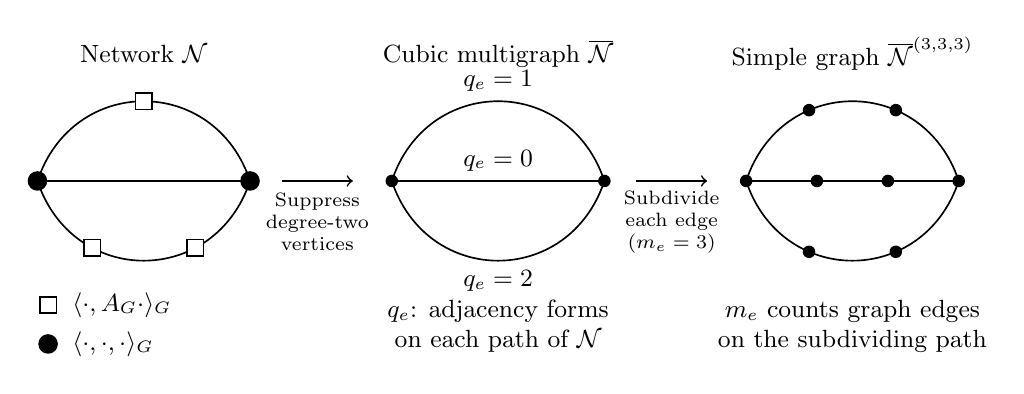
\begin{tikzpicture}[
  x=.9cm,y=.9cm,
  tensor/.style={circle,fill=black,inner sep=2.5pt},
  adjacency/.style={rectangle,draw,fill=white,minimum size=6pt,inner sep=0pt},
  vertex/.style={circle,fill=black,inner sep=1.6pt},
  every node/.style={font=\small},
  line width=.6pt,
]
\node at (1.5,1.8) {Network $\mathcal N$};
\draw (0,0)--(3,0);
\draw (0,0)..controls (.5,1.5) and (2.5,1.5)..(3,0)
  node[pos=.5,adjacency] {};
\draw (0,0)..controls (.5,-1.5) and (2.5,-1.5)..(3,0)
  node[pos=.3,adjacency] {} node[pos=.7,adjacency] {};
\node[tensor] at (0,0) {};
\node[tensor] at (3,0) {};
\node[adjacency] at (.15,-1.75) {};
\node[anchor=west] at (.35,-1.75) {$\langle\cdot,A_G\cdot\rangle_G$};
\node[tensor] at (.15,-2.3) {};
\node[anchor=west] at (.35,-2.3) {$\langle\cdot,\cdot,\cdot\rangle_G$};

\draw[->] (3.45,0)--(4.45,0);
\node[align=center,font=\scriptsize] at (3.95,-.58) {Suppress\\degree-two\\vertices};
\begin{scope}[xshift=4.5cm]
  \node at (1.5,1.8) {Cubic multigraph $\overline{\mathcal N}$};
  \draw (0,0)--(3,0) node[midway,above] {$q_e=0$};
  \draw (0,0)..controls (.5,1.5) and (2.5,1.5)..(3,0)
    node[midway,above] {$q_e=1$};
  \draw (0,0)..controls (.5,-1.5) and (2.5,-1.5)..(3,0)
    node[midway,below] {$q_e=2$};
  \node[vertex] at (0,0) {};
  \node[vertex] at (3,0) {};
  \node[align=center] at (1.5,-2.05) {$q_e$: adjacency forms\\on each path of $\mathcal N$};
\end{scope}

\draw[->] (8.45,0)--(9.45,0);
\node[align=center,font=\scriptsize] at (8.95,-.58) {Subdivide\\each edge\\($m_e=3$)};
\begin{scope}[xshift=9cm]
  \node at (1.5,1.8) {Simple graph $\overline{\mathcal N}^{(3,3,3)}$};
  \draw (0,0)--(3,0) node[pos=.333,vertex] {} node[pos=.667,vertex] {};
  \draw (0,0)..controls (.5,1.5) and (2.5,1.5)..(3,0)
    node[pos=.333,vertex] {} node[pos=.667,vertex] {};
  \draw (0,0)..controls (.5,-1.5) and (2.5,-1.5)..(3,0)
    node[pos=.333,vertex] {} node[pos=.667,vertex] {};
  \node[vertex] at (0,0) {};
  \node[vertex] at (3,0) {};
  \node[align=center] at (1.5,-2.05) {$m_e$ counts graph edges\\on the subdividing path};
\end{scope}
\end{tikzpicture}
\caption{A network, its cubic multigraph, and one simple subdivision.
The path represented by $e$ has $q_e$ adjacency forms and $q_e+1$ edges in $\mathcal N$;
a direct edge has $q_e=0$.
The subdivision on the right is chosen independently of the network paths,
with $m_e=3$ on every edge.
The expansions of $\val_G(\mathcal N)$ and $\hom(\overline{\mathcal N}^{\mathbf m},G)$
use the same coefficients $c_G(\overline{\mathcal N},\ell)$, with weights
$\prod_e\ell(e)^{q_e}$ and $\prod_e\ell(e)^{m_e}$, respectively.
Varying the lengths $m_e\geq3$ determines these coefficients and hence
the network value for every choice of $q_e\geq0$.}
\label{fig:network-subdivision}
\end{figure}


We next show that adjacency-image equivalence implies isomorphism for
graphs of nullity at most one.
For a graph $G$, we extend an orthonormal eigenbasis of $W_G$ to an
orthonormal eigenbasis $(u_i)_{i\in I}$ of $\R^{V(G)}$.
Let $\lambda_i$ be the eigenvalue of $u_i$ for each $i\in I$,
and let $I^{*}=\{i\in I:\lambda_i\ne0\}$.
Let $\gamma_1$ and $\gamma_3$ be the coefficient arrays of the
linear and trilinear forms in this eigenbasis, given by
\begin{equation}
  \label{eq:tensors}
  \begin{aligned}
  \gamma_1(i)&=\langle u_i\rangle_G, &
  \gamma_3(i,j,k)&=\langle u_i,u_j,u_k\rangle_G
  \end{aligned}
\end{equation}
for $i,j,k\in I$. For $x\in V(G)$, let $r_x=(u_i(x))_{i\in I}\in\R^I$ be
the row of $x$. These rows form an orthonormal basis of $\R^I$.
For $r\in\R^I$, let $r^{\otimes3}$ denote the array with entries
$r(i)r(j)r(k)$ for $i,j,k\in I$.
The rows satisfy
\begin{equation}
  \label{eq:rows}
  \begin{aligned}
  \gamma_3 &= \sum_{x \in V(G)} r_x^{\otimes 3}, &
  A_G(x,y) &= \sum_{i \in I} \lambda_i r_x(i) r_y(i).
  \end{aligned}
\end{equation}
We write $\gamma_3^{*}$ for the restriction of $\gamma_3$ to
indices in $I^{*}$.
In the eigenbasis $(u_i)_{i\in I^*}$ of $W_G$, the form
$\langle\cdot,\cdot,\cdot\rangle_G$ has coefficient array $\gamma_3^*$.
When $G$ has nullity one, we index the basis so that $I=I^*\sqcup\{0\}$
and $u_0$ spans $\ker A_G$.
In particular, $\gamma_1(0)=\sum_{x\in V(G)}u_0(x)$.
For such a graph, let $\tilde{r}_x=(u_i(x))_{i\in I^*}$ be
its reduced row at $x$.
Since $\tilde{r}_x$ is $r_x$ with its kernel coordinate omitted,
orthonormality of the rows gives
\begin{equation}\label{eq:gram}
 \langle\tilde{r}_x,\tilde{r}_y\rangle=\delta_{xy}-u_0(x)u_0(y).
\end{equation}
The coefficients of $\gamma_3$ outside
$\gamma_3^*$ are the $\gamma_3(i,j,k)$ with at least one
index equal to $0$.

If $G$ has nullity one and $|\supp u_0|>2$, then
\begin{equation}\label{eq:support-neighbourhoods}
 N_G(x)\ne N_G(y)\quad\text{for distinct }x,y\in\supp u_0.
\end{equation}
Indeed, for the standard coordinate vectors $e_x,e_y\in\R^{V(G)}$,
$e_x-e_y$ has support of size two, so it is not a scalar multiple of
$u_0$. Thus $A_G(e_x-e_y)\ne0$, which gives
\cref{eq:support-neighbourhoods}.

The final assertion of the next lemma is a special case of uniqueness of
orthogonal tensor decompositions~\cite[Theorem~3.2]{ZhangGolub2001}.
\begin{lemma}\label{lem:odeco}
 Let $X,I$ be finite sets, and let $R\in\R^{X\times I}$ be a matrix
 with orthonormal columns. Write $r_x\in\R^I$ for its row indexed by
 $x\in X$, and define $\kappa:\R^I\to\R$ by
 $\kappa(\xi)=\sum_{x\in X}\langle r_x,\xi\rangle^3$.
 Then
 \begin{equation}\label{eq:cubic-unit-rows}
  \{\xi:\lVert \xi\rVert=1,\ \kappa(\xi)=1\}
  =\{r_x:\lVert r_x\rVert=1\}.
 \end{equation}
 In particular, if $(r_x)_{x\in X}$ and $(r'_y)_{y\in Y}$ are
 orthonormal bases of the same Euclidean space and
 $\sum_x r_x^{\otimes3}=\sum_y(r'_y)^{\otimes3}$, then there is a
 bijection $\pi:X\to Y$ with $r'_{\pi(x)}=r_x$ for every $x\in X$.
\end{lemma}
\begin{proof}
 Let $\xi$ be a unit vector and put $c=R\xi$.
 Since the columns of $R$ are orthonormal, we have $\sum_xc_x^2=1$. Hence
 \begin{equation}\label{eq:cubic-unit-defect}
  1-\kappa(\xi)=\sum_x c_x^2(1-c_x)\geq0.
 \end{equation}
 Equality holds exactly when $c=e_x$ for some $x$,
 where $e_x$ is the standard coordinate vector.
 Then $\xi=R^{\top}c=r_x$.
 Conversely, if $\lVert r_x\rVert=1$, then $Rr_x$ is a unit vector
 whose $x$-coordinate is $1$, so $Rr_x=e_x$ and
 $\kappa(r_x)=1$. This proves \cref{eq:cubic-unit-rows}.
 The final assertion follows because equal cubic tensors identify the
 same set of unit rows.
\end{proof}
\begin{lemma}\label{lem:four-vertex-reconstruction}
Let $G,G'$ have nullity one and orthonormal eigenbases
$(u_i)_{i\in I}$ and $(u'_i)_{i\in I}$, respectively, with the same
corresponding eigenvalues $\lambda_i$.
Index both bases by $I=I^*\sqcup\{0\}$, with kernel vectors $u_0,u'_0$,
and write $\tilde{r}_x,\tilde{r}'_y\in\R^{I^*}$ for the reduced rows.
Suppose that $|\supp u_0|=|\supp u'_0|=4$ and
$\sum_xu_0(x)=\sum_yu'_0(y)=0$.
Suppose also that the reduced rows outside these supports agree as multisets and
$\sum_{x\in\supp u_0}\tilde{r}_x=\sum_{y\in\supp u'_0}\tilde{r}'_y$.
Then the reduced rows on the two supports agree as multisets.
\end{lemma}
\begin{proof}
  The rows outside each support are orthonormal by \cref{eq:gram}.
  We relabel the vertices of $G'$ outside $\supp u'_0$ so that
  $\tilde{r}'_z=\tilde{r}_z$ for every $z\notin\supp u_0$.
  We first show that $\supp u_0$ admits at least two distinct
  partitions into pairs on which $u_0$ sums to zero.
  For $w\in V(G)$, let $N_0(w)=N_G(w)\cap\supp u_0$.
  Then $\sum_{x\in N_0(w)}u_0(x)=(A_Gu_0)(w)=0$.
  If a nonempty proper subset $T$ of $\supp u_0$ satisfies
  $\sum_{x\in T}u_0(x)=0$, then $|T|=2$ and
  $\sum_{x\in\supp u_0\setminus T}u_0(x)=0$, since the four support
  entries are nonzero and sum to zero.
  Choose distinct $x,y\in\supp u_0$.
  By \cref{eq:support-neighbourhoods}, there is a vertex $w_1$ for which
  $N_0(w_1)$ contains exactly one of $x,y$.
  Thus $N_0(w_1)$ is nonempty and proper, and
  $\{N_0(w_1),\supp u_0\setminus N_0(w_1)\}$ is a first partition
  into zero-sum pairs.
  The two vertices of $N_0(w_1)$ also have different neighbourhoods,
  so there is a vertex $w_2$ for which $N_0(w_2)$ contains exactly
  one of them. Again $N_0(w_2)$ is nonempty and proper, so
  $\{N_0(w_2),\supp u_0\setminus N_0(w_2)\}$ is a partition into
  zero-sum pairs. It differs from the first partition because its
  two pairs separate the vertices of $N_0(w_1)$.

  We label $\supp u_0=\{a,b,c,d\}$ so that $u_0$ sums to zero
  on each pair in the two partitions
  $\{\{a,c\},\{b,d\}\}$ and $\{\{a,d\},\{b,c\}\}$.
  Since $u_0$ sums to zero on each of $\{a,c\}$, $\{a,d\}$ and
  $\{b,c\}$, we have
  $u_0(c)=u_0(d)=-u_0(a)=-u_0(b)$.
  Since $u_0$ is a unit vector, a choice of sign gives
  \begin{equation}
    \label{eq:support4}
    \begin{aligned}
      u_0(a)&=u_0(b)=\frac12, &
      u_0(c)&=u_0(d)=-\frac12.
    \end{aligned}
  \end{equation}
  Every $N_0(w)$ is then empty, equal to $\supp u_0$, or one of
  $\{a,c\}$, $\{a,d\}$, $\{b,c\}$, $\{b,d\}$.
  Since $\sum_yu'_0(y)=0$ and $|\supp u'_0|=4$, the same argument
  gives the nonzero entries $(\tfrac12,\tfrac12,-\tfrac12,-\tfrac12)$
  for $u'_0$, up to permutation and a choice of sign.

  We now show that $\{\tilde{r}_x:x\in\supp u_0\}$ and
  $\{\tilde{r}'_y:y\in\supp u'_0\}$ have the same centre and span the
  same affine plane.
  We choose the sign of $u'_0$ and label
  $\supp u'_0=\{a',b',c',d'\}$ so that
  $(u'_0(a'),u'_0(b'),u'_0(c'),u'_0(d'))=$
  $(\tfrac12,\tfrac12,-\tfrac12,-\tfrac12)$.
  Let $\sigma = \tilde{r}_a + \tilde{r}_b$,
  $f = (\tilde{r}_a - \tilde{r}_b)/\sqrt{2}$ and
  $g = (\tilde{r}_c - \tilde{r}_d)/\sqrt{2}$.
  Let $\sigma',f',g'$ be given by the formulas for $\sigma,f,g$ with
  primed vertices and rows.
  By \cref{eq:gram} and
  \cref{eq:support4}, the vectors $\sigma,f,g$ together with
  $(\tilde{r}_z)_{z\in V(G)\setminus\supp u_0}$ form an orthonormal basis of
  $\R^{I^*}$. Since $u_0$ is orthogonal to every $u_i$ with $i\in I^*$,
  we have $\sum_xu_0(x)\tilde{r}_x=0$.
  Substituting \cref{eq:support4} gives
  $\tilde{r}_a+\tilde{r}_b=\tilde{r}_c+\tilde{r}_d$, so $\sigma=\tilde{r}_c+\tilde{r}_d$. Hence
  \begin{equation}
    \label{eq:special-rows}
    \begin{aligned}
    \tilde{r}_a &= \frac{1}{2} \sigma + \frac{1}{\sqrt{2}} f, &
    \tilde{r}_b &= \frac{1}{2} \sigma - \frac{1}{\sqrt{2}} f, &
    \tilde{r}_c &= \frac{1}{2} \sigma + \frac{1}{\sqrt{2}} g, &
    \tilde{r}_d &= \frac{1}{2} \sigma - \frac{1}{\sqrt{2}} g.
    \end{aligned}
  \end{equation}
  The centres of $\{\tilde{r}_a,\tilde{r}_b,\tilde{r}_c,\tilde{r}_d\}$ and
  $\{\tilde{r}'_{a'},\tilde{r}'_{b'},\tilde{r}'_{c'},\tilde{r}'_{d'}\}$ are their averages
  $\sigma/2$ and $\sigma'/2$. By the assumed equality of the support-row sums,
  \begin{equation}\label{eq:quartet-offset}
    \frac12\sigma'=\frac14\sum_{y\in\supp u'_0}\tilde{r}'_y
    =\frac14\sum_{x\in\supp u_0}\tilde{r}_x=\frac12\sigma.
  \end{equation}
  Since $\sigma'=\sigma$ and $\tilde{r}'_z=\tilde{r}_z$ for
  $z\notin\supp u_0$, the orthonormal bases
  $\{\sigma,f,g\}\cup\{\tilde{r}_z:z\notin\supp u_0\}$ and
  $\{\sigma',f',g'\}\cup\{\tilde{r}'_z:z\notin\supp u'_0\}$ give
  \begin{equation}\label{eq:quartet-plane}
   \spn(f,g)
   =\spn\bigl(\{\tilde{r}_z:z\notin\supp u_0\}\cup\{\sigma\}\bigr)^\perp
   =\spn(f',g').
  \end{equation}
  Thus both sets of four vectors have affine span $\sigma/2+\spn(f,g)$.

  We now use the entries of $A_{G'}$ to show that $f'\in\{\pm f,\pm g\}$.
  Let $\alpha,\beta\in\R$ be the coefficients in $f'=\alpha f+\beta g$.
  Since $(f,g)$ is orthonormal and $f'$ is a unit vector,
  $\alpha^2+\beta^2=1$.
  For each $z\in V(G)\setminus\supp u_0$, let
  $\Delta_z^f=A_G(a,z)-A_G(b,z)$ and
  $\Delta_z^g=A_G(c,z)-A_G(d,z)$.
  By \cref{eq:rows,eq:special-rows},
  \begin{equation}\label{eq:quartet-adjacency}
    \begin{aligned}
      \sqrt2 f^{\top}\diag(\lambda_i)_{i\in I^*}\tilde{r}_z &= \Delta_z^f,\\
      \sqrt2 g^{\top}\diag(\lambda_i)_{i\in I^*}\tilde{r}_z &= \Delta_z^g,\\
      \sigma^{\top}\diag(\lambda_i)_{i\in I^*}\tilde{r}_z &= A_G(a,z)+A_G(b,z).
    \end{aligned}
  \end{equation}
  Since $\sigma'=\sigma$ and $f'=\alpha f+\beta g$, we have
  $\tilde{r}'_{a'}=\tfrac12\sigma+\tfrac1{\sqrt2}(\alpha f+\beta g)$
  by \cref{eq:special-rows} for $G'$.
  Substituting this formula for $\tilde{r}'_{a'}$ and $\tilde{r}'_z=\tilde{r}_z$ into
  the second identity in \cref{eq:rows} for $G'$, and using
  \cref{eq:quartet-adjacency}, gives
  \begin{equation}
    \label{eq:integrality}
    A_{G'}(a', z) = \frac{1}{2}\bigl(A_G(a,z)+A_G(b,z)\bigr)
      + \frac{1}{2}(\alpha\Delta_z^f+\beta\Delta_z^g)\in\{0,1\}.
  \end{equation}

  We have $\alpha\beta=0$ whenever a vertex $z\notin\supp u_0$ satisfies
  \begin{equation}\label{eq:quartet-probe}
    A_G(a,z)+A_G(b,z)=A_G(c,z)+A_G(d,z)=1.
  \end{equation}
  Indeed, then $\Delta_z^f,\Delta_z^g\in\{\pm1\}$ and
  $A_G(a,z)+A_G(b,z)=1$, so \cref{eq:integrality} gives
  $\alpha\Delta_z^f+\beta\Delta_z^g=\pm1$.
  Squaring gives
  $1=\alpha^2+\beta^2+2\alpha\beta\Delta_z^f\Delta_z^g
  =1+2\alpha\beta\Delta_z^f\Delta_z^g$, so $\alpha\beta=0$.
  \Cref{fig:quartet-geometry} gives a geometric interpretation of this calculation.

  \begin{figure}[tb]
\centering
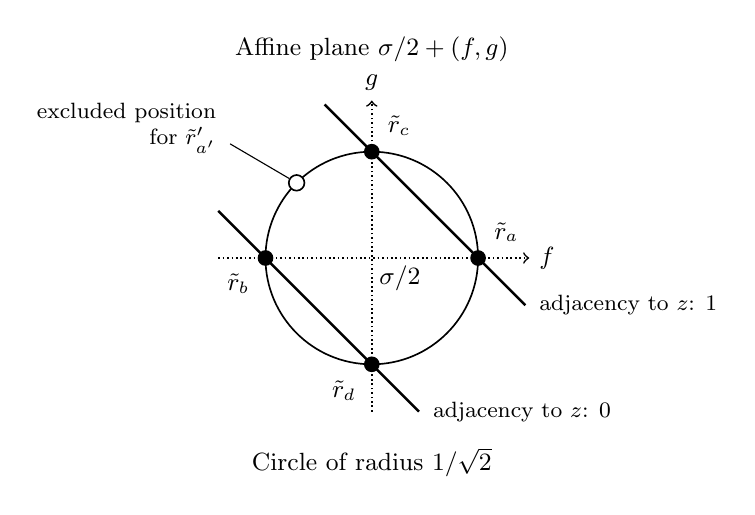
\begin{tikzpicture}[
  every node/.style={font=\small},
  point/.style={circle,fill=black,inner sep=2pt},
  candidate/.style={circle,draw,fill=white,inner sep=2pt},
  line width=.6pt,
]
\node at (0,2.65) {Affine plane $\sigma/2+\spn(f,g)$};
\draw[densely dotted,->] (-1.95,0)--(2,0) node[right] {$f$};
\draw[densely dotted,->] (0,-1.95)--(0,2) node[above] {$g$};
\draw (0,0) circle[radius=1.35];
\draw[line width=.9pt] (-.6,1.95)--(1.95,-.6);
\node[anchor=west,font=\footnotesize] at (2,-.6) {adjacency to $z$: $1$};
\draw[line width=.9pt] (-1.95,.6)--(.6,-1.95);
\node[anchor=west,font=\footnotesize] at (.65,-1.95) {adjacency to $z$: $0$};
\node[fill=white,inner sep=1pt,anchor=north west] at (.05,-.05) {$\sigma/2$};
\node[point,label=above right:$\tilde{r}_a$] at (1.35,0) {};
\node[point,label=below left:$\tilde{r}_b$] at (-1.35,0) {};
\node[point,label=above right:$\tilde{r}_c$] at (0,1.35) {};
\node[point,label=below left:$\tilde{r}_d$] at (0,-1.35) {};
\node[candidate] (excluded) at (135:1.35) {};
\node[anchor=east,align=right,font=\footnotesize] at (-1.85,1.65)
  {excluded position\\for $\tilde{r}'_{a'}$};
\draw[thin] (-1.8,1.45)--(excluded);
\node at (0,-2.6) {Circle of radius $1/\sqrt2$};
\end{tikzpicture}
\caption{Geometric interpretation of the calculation giving $\alpha\beta=0$.
The figure assumes that $z\in V(G)\setminus\supp u_0$ is adjacent to $a,c$
and not to $b,d$; the other cases of \cref{eq:quartet-probe} are symmetric.
For a candidate $\tilde{r}'_{a'}=\sigma/2+(\alpha f+\beta g)/\sqrt2$,
the circle gives $\alpha^2+\beta^2=1$.
By \cref{eq:integrality}, the two lines have equations
$\alpha+\beta=1$ and $\alpha+\beta=-1$.
Squaring either equation and subtracting the circle equation gives
$2\alpha\beta=0$. The hollow point is on the circle but off both lines,
so \cref{eq:integrality} excludes it.}
\label{fig:quartet-geometry}
\end{figure}


  We show that \cref{eq:quartet-probe} holds for some
  $z\in V(G)\setminus\supp u_0$. Otherwise, the list of
  possible sets $N_0(z)$ implies
  $N_0(z)\in\{\varnothing,\supp u_0\}$ for every
  $z\notin\supp u_0$.
  For $w\in\supp u_0$, we have $w\notin N_0(w)$ because $G$ has no loops.
  Thus a nonempty $N_0(w)$ must be one of
  $\{a,c\}$, $\{a,d\}$, $\{b,c\}$ and $\{b,d\}$.
  Every nonisolated vertex in the graph induced by $\supp u_0$
  therefore has exactly two neighbours, one in $\{a,b\}$ and one in
  $\{c,d\}$. A nonisolated vertex in $\{a,b\}$ is adjacent to the
  other vertex of $\{a,b\}$; the same holds for $\{c,d\}$.
  If the induced graph has an edge, it therefore also has an edge
  between $\{a,b\}$ and $\{c,d\}$.
  Each of these two sets then contains a nonisolated vertex and hence
  both its vertices are nonisolated. All four vertices have degree two,
  so the induced graph is a cycle of length four.
  Thus either the induced graph is edgeless, or it is a four-cycle.
  There are distinct $x,y\in\supp u_0$ with $N_0(x)=N_0(y)$:
  any two vertices in the edgeless case, or opposite vertices in the
  four-cycle case. Also
  $N_G(x)\setminus\supp u_0=N_G(y)\setminus\supp u_0$, because every
  vertex outside the support is adjacent to all four support vertices
  or to none. Hence $N_G(x)=N_G(y)$, contradicting
  $N_G(x)\ne N_G(y)$ for distinct $x,y\in\supp u_0$.

  A vertex $z\notin\supp u_0$ satisfying \cref{eq:quartet-probe}
  exists, so $\alpha\beta=0$. Together with $\alpha^2+\beta^2=1$,
  this gives $(\alpha,\beta)\in\{(1,0),(-1,0),(0,1),(0,-1)\}$,
  hence $f'\in\{\pm f,\pm g\}$. Since $(f',g')$ is orthonormal in
  $\spn(f,g)$, we have $\{\pm f',\pm g'\}=\{\pm f,\pm g\}$.
  Together with $\sigma'=\sigma$, \cref{eq:special-rows} now gives
  \begin{equation}\label{eq:quartet-row-equality}
    \{\tilde{r}_a,\tilde{r}_b,\tilde{r}_c,\tilde{r}_d\}
    =\{\tilde{r}'_{a'},\tilde{r}'_{b'},\tilde{r}'_{c'},\tilde{r}'_{d'}\}.
  \end{equation}
  The four vectors on each side are distinct by \cref{eq:special-rows},
  so they agree as multisets.
\end{proof}

\begin{lemma}\label{lem:reconstruction}
 Let $G$ have nullity at most one, and let $G'$ be a graph.
 If $G\sim_{\mathrm{im}}G'$, then $G\cong G'$.
\end{lemma}
\begin{proof}
  We fix a bijective linear map $U:W_G\to W_{G'}$ witnessing
  $G\sim_{\mathrm{im}}G'$.
  The graphs $G$ and $G'$ have the same number of vertices because
  $G\sim_{\mathrm{im}}G'$. The map $U$ intertwines
  $A_G|_{W_G}$ with $A_{G'}|_{W_{G'}}$, so their nonzero eigenvalues agree
  with multiplicities. Thus their zero multiplicities also agree,
  and both graphs have the same nullity, at most one.
  We fix an orthonormal eigenbasis
  $(u_i)_{i\in I}$ of $\R^{V(G)}$.
  Let $(u'_i)_{i\in I}$ be an orthonormal eigenbasis of $\R^{V(G')}$
  with $u'_i=Uu_i$ for every $i\in I^*$.
  Then $u_i$ and $u'_i$ have the same eigenvalue $\lambda_i$ for every
  $i\in I$. We use primes for quantities associated with $G'$.
  By \cref{eq:adjacency-image-equivalence} and
  \cref{eq:image-sum-transport}, for $i,j,k\in I^*$,
  \begin{equation}\label{eq:transported-tensors}
    \begin{aligned}
      \gamma'_1(i)&=\langle Uu_i\rangle_{G'}
        =\langle u_i\rangle_G=\gamma_1(i),\\
      \gamma'_3(i,j,k)&=\langle Uu_i,Uu_j,Uu_k\rangle_{G'}
        =\langle u_i,u_j,u_k\rangle_G=\gamma_3(i,j,k).
    \end{aligned}
  \end{equation}
  For $x\in V(G)$ and $y\in V(G')$, let
  $\tilde{r}_x=(u_i(x))_{i\in I^*}$ and
  $\tilde{r}'_y=(u'_i(y))_{i\in I^*}$ be the reduced rows.
  A bijection $\pi:V(G)\to V(G')$ with $\tilde{r}'_{\pi(x)}=\tilde{r}_x$ is a
  graph isomorphism. The zero-eigenvalue terms in the second identity of
  \cref{eq:rows} vanish, so for $x,y\in V(G)$ we have
  \begin{equation}\label{eq:row-isomorphism}
    A_{G'}(\pi(x),\pi(y))
    =\sum_{i\in I^*}\lambda_i\tilde{r}'_{\pi(x)}(i)\tilde{r}'_{\pi(y)}(i)
    =\sum_{i\in I^*}\lambda_i\tilde{r}_x(i)\tilde{r}_y(i)=A_G(x,y).
  \end{equation}
  If $\gamma_3=\gamma'_3$, then by \cref{lem:odeco} there is a
  bijection $\pi$ with $r'_{\pi(x)}=r_x$, hence $\tilde{r}'_{\pi(x)}=\tilde{r}_x$.
  If the graphs are nonsingular, then $I^*=I$, so
  \cref{eq:transported-tensors} already gives $\gamma_3=\gamma'_3$
  and hence $G\cong G'$.

  We therefore assume that both graphs have nullity one.
  We index $(u_i)$ and $(u'_i)$ so that $I=I^*\sqcup\{0\}$, with unit kernel
  vectors $u_0,u'_0$. Once $(u_i)_{i\in I^*}$ and $(u'_i)_{i\in I^*}$ are fixed,
  the only remaining choices are the signs of $u_0$ and $u'_0$.
  We first compare the coefficients involving index $0$, which are
  not compared in \cref{eq:transported-tensors}.
  By symmetry of $\gamma_3$, the \emph{missing coefficients} are
  $\gamma_1(0)$, $\gamma_3(0,0,0)$, $\gamma_3(0,0,k)$ and
  $\gamma_3(0,j,k)$ for $j,k\in I^*$.
  We seek a choice of signs for $u_0,u'_0$ for which these coefficients
  agree with their primed counterparts. If these coefficients agree, then
  \cref{eq:transported-tensors} gives $\gamma_3=\gamma'_3$,
  and \cref{lem:odeco} gives a vertex bijection $\pi$ satisfying
  $\tilde{r}'_{\pi(v)}=\tilde{r}_v$ for every $v\in V(G)$.
  Replacing $u_0$ by $-u_0$ negates $\gamma_1(0)$,
  $\gamma_3(0,0,0)$ and $\gamma_3(0,j,k)$, while leaving
  $\gamma_3(0,0,k)$ unchanged. Replacing $u'_0$ by $-u'_0$
  has the same effect on the primed coefficients.

  The arrays $\gamma_1,\gamma_3$ satisfy the following identities for all $i,j,k,l\in I$
  because the vectors $r_x$ form an orthonormal basis:
  \begin{gather}
    \label{eq:id-norm}
    \sum_{m \in I} \gamma_1(m)^{2} = |V(G)|, \\
    \label{eq:id-unit}
    \sum_{m \in I} \gamma_1(m) \gamma_3(m,j,k) = \delta_{jk}, \\
    \label{eq:id-trace}
    \sum_{m \in I} \gamma_3(j,m,m) = \gamma_1(j), \\
    \label{eq:id-assoc}
    \sum_{m \in I} \gamma_3(i,j,m) \gamma_3(m,k,l)
      = \sum_{x \in V(G)} u_i(x) u_j(x) u_k(x) u_l(x).
  \end{gather}
  Separating the term $m=0$ in \cref{eq:id-trace} gives, for $k\in I^*$,
  \begin{equation}
    \label{eq:trace-completion}
    \begin{aligned}
      \gamma_3(0,0,k) &= \gamma_1(k) - \sum_{i\in I^*}\gamma_3(k,i,i),\\
      \gamma_3(0,0,0) &= \gamma_1(0) - \sum_{i\in I^*}\gamma_3(0,i,i).
    \end{aligned}
  \end{equation}
  The first identity involves only coefficients at indices in $I^*$ on
  the right-hand side, so $\gamma'_3(0,0,k)=\gamma_3(0,0,k)$ by
  \cref{eq:transported-tensors}. The second determines
  $\gamma_3(0,0,0)$ from $\gamma_1(0)$ and the coefficients
  $\gamma_3(0,j,k)$. Thus agreement of all missing coefficients
  reduces to agreement of $\gamma_1(0)$ and $\gamma_3(0,j,k)$
  with their primed counterparts.

  For the case analysis, let $\mathsf C_0$ be the symmetric
  $I^*\times I^*$ matrix defined by
  \begin{equation}\label{eq:unknowns}
    \mathsf C_0(j,k) = \gamma_3(0,j,k).
  \end{equation}
  Separating the term $m=0$ in \cref{eq:id-norm} gives
  $\gamma_1(0)^2=|V(G)|-\sum_{i\in I^*}\gamma_1(i)^2$, so
  $\gamma_1(0)^2=(\gamma'_1(0))^2$ by \cref{eq:transported-tensors}.
  We divide the remaining proof into $\gamma_1(0)\ne0$ (Case A)
  and $\gamma_1(0)=0$ (Case B).
  Within Case B, we distinguish $\rank\mathsf C_0\geq3$ (Case B1)
  from $\rank\mathsf C_0\leq2$ (Case B2).
  In Cases A and B1, we show that a choice of sign for $u'_0$ gives
  $\gamma'_1(0)=\gamma_1(0)$ and $\mathsf C'_0=\mathsf C_0$.
  In Case B2, we use the graph structure to show that $u_0$ has
  support of size two or four. In both subcases, we show directly
  that $(\tilde{r}_x)_{x\in V(G)}$ and $(\tilde{r}'_y)_{y\in V(G')}$ agree as multisets.

  \emph{Case A: $\gamma_1(0) \neq 0$.} We choose the sign of $u'_0$ so
  that $\gamma'_1(0)=\gamma_1(0)$. Separating the term $m=0$ in
  \cref{eq:id-unit} gives
  \begin{equation}
    \label{eq:caseA}
    \gamma_1(0) \mathsf{C}_0(j,k) = \delta_{jk} - \sum_{i \in I^{*}} \gamma_1(i) \gamma_3(i,j,k).
  \end{equation}
  The right-hand side for $G'$ equals the right-hand side for $G$ by
  \cref{eq:transported-tensors}, and dividing by
  $\gamma_1(0)=\gamma'_1(0)\neq0$ gives $\mathsf C'_0=\mathsf C_0$.
  Hence $\gamma_3=\gamma'_3$.

  \emph{Case B: $\gamma_1(0) = 0$.} Then $\gamma'_1(0)=0$, since
  $(\gamma'_1(0))^2=\gamma_1(0)^2$. Here \cref{eq:id-unit} no longer
  determines $\mathsf C_0$.

  \emph{Case B1: $\rank \mathsf{C}_0 \geq 3$.} We show that
  $\mathsf C'_0=\pm\mathsf{C}_0$ by comparing their $2\times2$ minors.
  For $i,j,k,l \in I^{*}$ let $Q(i,j;k,l)$ be the sum of the terms with
  $m\neq0$ in \cref{eq:id-assoc},
  \begin{equation}\label{eq:q-tensor}
   Q(i,j;k,l) = \sum_{m \in I^{*}} \gamma_3(i,j,m) \gamma_3(m,k,l),
  \end{equation}
  which involves only $\gamma_3^*$.
  Separating the term $m=0$ in \cref{eq:id-assoc} gives
  \begin{equation}
    \label{eq:assoc-split}
    \mathsf{C}_0(i,j)\mathsf{C}_0(k,l)+Q(i,j;k,l)
    =\sum_{x \in V(G)} u_i(x) u_j(x) u_k(x) u_l(x).
  \end{equation}
  The right-hand side is symmetric in $(i,j,k,l)$, so subtracting from
  \cref{eq:assoc-split} the same identity with $j$ and $k$ exchanged
  gives
  \begin{equation}
    \label{eq:minors}
    \mathsf{C}_0(i,j) \mathsf{C}_0(k,l) - \mathsf{C}_0(i,k) \mathsf{C}_0(j,l) = Q(i,k;j,l) - Q(i,j;k,l).
  \end{equation}
  The left-hand side is the minor of $\mathsf{C}_0$ with rows $i,l$ and
  columns $j,k$. The right-hand side involves only $\gamma_3^*$,
  which $G$ and $G'$ share by \cref{eq:transported-tensors}. Hence each
  $2\times2$ minor of $\mathsf C'_0$ equals the minor of
  $\mathsf{C}_0$ with the same rows and columns.
  Thus the exterior squares of $\mathsf C_0$ and $\mathsf C'_0$ are equal.
  Since $\rank\mathsf C_0\geq3$, \cite[Corollary~4.1]{Greenhill1999}
  gives $\mathsf C'_0=\pm\mathsf C_0$.
  We choose the sign of $u'_0$ so that $\mathsf C'_0=\mathsf{C}_0$.
  Hence $\gamma_3=\gamma'_3$.

  \emph{Case B2: $\rank \mathsf{C}_0 \leq 2$.} We show that
  $\{\tilde{r}_z:z\notin\supp u_0\}=\{\tilde{r}'_z:z\notin\supp u'_0\}$.
  Let $R$ be the matrix with rows $\tilde{r}_x$. Its columns are
  orthonormal, and \cref{eq:gram} gives
  $\lVert\tilde{r}_x\rVert^2=1-u_0(x)^2$.
  Thus $\tilde{r}_x$ is a unit vector exactly when $x\notin\supp u_0$.
  The same holds for $\tilde{r}'_y$ and $\supp u'_0$.
  Let $\kappa$ and $\kappa'$ be the cubic forms with coefficient
  arrays $\gamma_3^*$ and $(\gamma'_3)^*$, respectively, so
  \begin{equation}\label{eq:reduced-cubic}
   \kappa(\xi)=\sum_x\langle\tilde{r}_x,\xi\rangle^3
   =\sum_y\langle\tilde{r}'_y,\xi\rangle^3=\kappa'(\xi)
  \end{equation}
  by \cref{eq:transported-tensors}.
  By \cref{lem:odeco} and \cref{eq:reduced-cubic},
  \begin{equation}\label{eq:outside-rows}
   \{\tilde{r}_z:z\notin\supp u_0\}
   =\{\xi:\lVert \xi\rVert=1,\ \kappa(\xi)=1\}
   =\{\tilde{r}'_z:z\notin\supp u'_0\}.
  \end{equation}
  Each of these row families is orthonormal by \cref{eq:gram}, so its
  members are distinct. Since $G$ and $G'$ have the same number of
  vertices, \cref{eq:outside-rows} also gives
  $|\supp u'_0|=|\supp u_0|$.
  We relabel the vertices of $G'$ outside $\supp u'_0$ so that
  $\tilde{r}'_z=\tilde{r}_z$ for every $z\notin\supp u_0$.

  It remains to compare $(\tilde{r}_x)_{x\in\supp u_0}$ and
  $(\tilde{r}'_y)_{y\in\supp u'_0}$ as multisets.
  Their sums agree: by
  \cref{eq:transported-tensors} and \cref{eq:outside-rows},
  \begin{equation}\label{eq:support-row-sum}
    \sum_{x\in\supp u_0}\tilde{r}_x
    = (\gamma_1(i))_{i\in I^*}-\sum_{z\notin\supp u_0}\tilde{r}_z
    = \sum_{y\in\supp u'_0}\tilde{r}'_y.
  \end{equation}
  We claim that
  \begin{equation}\label{eq:kernel-support-sizes}
    |\supp u_0|\in\{2,4\}.
  \end{equation}
  Since $\mathsf{C}_0 = R^{\top} \diag(u_0) R$ and
  $\rank R=|V(G)|-1$, Sylvester's rank inequality gives
  $|\supp u_0| \leq \rank \mathsf{C}_0 + 2 \leq 4$.
  The support has at least two vertices because $u_0\ne0$ and
  $\gamma_1(0)=0$.
  Suppose it has three vertices. For every nonempty proper subset
  $T$ of $\supp u_0$, we have $\sum_{x\in T}u_0(x)\ne0$, since
  the three entries are nonzero and their sum is zero.
  The equation $(A_Gu_0)(w)=\sum_{x\in N_G(w)}u_0(x)=0$ therefore
  forces every vertex $w$ to be adjacent to all three support
  vertices or to none. Thus $N_G(x)=N_G(y)$ for any two distinct
  support vertices $x,y$, contradicting \cref{eq:support-neighbourhoods}.

  \emph{Case B2 with $|\supp u_0|=2$.} Write
  $\supp u_0=\{x,y\}$ and $\supp u'_0=\{x',y'\}$.
  Since $u_0(x)=-u_0(y)\ne0$, we have
  $0=\langle u_0,u_i\rangle_G=u_0(x)(u_i(x)-u_i(y))$ for all $i\in I^*$,
  so $\tilde{r}_x=\tilde{r}_y$. The same holds for $u'_0$.
  By \cref{eq:support-row-sum},
  $\tilde{r}_x+\tilde{r}_y=\tilde{r}'_{x'}+\tilde{r}'_{y'}$, hence
  $\tilde{r}_x=\tilde{r}_y=\tilde{r}'_{x'}=\tilde{r}'_{y'}$.
  Together with \cref{eq:outside-rows}, this gives a vertex bijection
  $\pi$ satisfying $\tilde{r}'_{\pi(v)}=\tilde{r}_v$ for every $v\in V(G)$.
  Hence $G\cong G'$ by \cref{eq:row-isomorphism}.

  \emph{Case B2 with $|\supp u_0|=4$.}
  Both kernel vectors have support of size four and sum zero.
  Their outside rows agree by \cref{eq:outside-rows}, and their
  support-row sums agree by \cref{eq:support-row-sum}.
  Thus \cref{lem:four-vertex-reconstruction} identifies the remaining
  reduced rows as multisets.
  Combining the two correspondences gives a bijection $\pi$ with
  $\tilde{r}'_{\pi(x)}=\tilde{r}_x$, which is an isomorphism by \cref{eq:row-isomorphism}.
\end{proof}

\begin{proof}[Proof of \cref{thm:main}]

 Suppose $G\equiv_{\mathcal D_3}G'$. By \cref{lem:characterisation},
 $G\sim_{\mathrm{im}}G'$. Hence $G\cong G'$ by \cref{lem:reconstruction}.
 Conversely, an isomorphism $\pi:G\to G'$ gives a bijection
 $\varphi\mapsto\pi\circ\varphi$ between homomorphisms $F\to G$ and $F\to G'$
 for every $F$, so $G\equiv_{\mathcal D_3}G'$.
 A graph with simple spectrum has nullity at most one, because a real
 symmetric matrix with pairwise distinct eigenvalues has zero as an
 eigenvalue at most once; hence $\mathcal D_3$ is complete on simple
 spectrum.
\end{proof}

\begin{remark}\label{rem:nullity-bound}
The nullity bound in \cref{thm:main} cannot be raised to three.
Let $B$ be the cricket graph shown in \cref{fig:cricket}.
The graphs $\CFI_0(B)$ and $\CFI_1(B)$ defined in
\cref{eq:ss-cfi-definition} each have $14$ vertices.
A direct calculation gives nullity three for both graphs.
They are non-isomorphic and homomorphism indistinguishable over
$\mathcal D_3$ by~\cite[Corollary~3.7 and the proof of Corollary~4.2]{Roberson2026}.
It remains open whether \cref{thm:main} extends to graphs of nullity two.
An exhaustive search found no pair of non-isomorphic graphs of nullity two
on at most $11$ vertices that are homomorphism indistinguishable over
$\mathcal D_3$.
\end{remark}

\begin{figure}[tb]
\centering
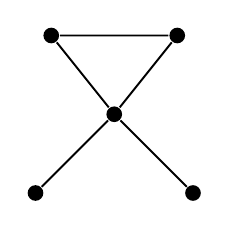
\begin{tikzpicture}[
  vertex/.style={circle,fill,inner sep=2pt},
  line width=.7pt,
]
\node[vertex] (centre) at (0,0) {};
\node[vertex] (upperleft) at (-.8,1) {};
\node[vertex] (upperright) at (.8,1) {};
\node[vertex] (lowerleft) at (-1,-1) {};
\node[vertex] (lowerright) at (1,-1) {};
\draw (centre)--(upperleft)--(upperright)--(centre);
\draw (lowerleft)--(centre)--(lowerright);
\end{tikzpicture}
\caption{The cricket graph $B$.}
\label{fig:cricket}
\end{figure}

